\apendice{Documentación de usuario}

\section{Introducción}

En esta sección vamos a detallar los requisitos necesarios para la instalación y uso del sistema, así como el manual de cómo realizar dicha instalación. También se desarrollará un manual de uso. Todo ello enfocado al usuario final.

\section{Requisitos de usuarios}

\begin{itemize}
\item
	Dispositivo Android con una versión igual o superior a Android Jelly Bean o Android 4.1, para el uso de la aplicación.
\item
	Dispositivo de bajo consumo (recomendado) o PC con conexión a Internet, y con Python 3 instalado, para albergar el servidor.
\item
	Es necesario que el dispositivo Android y el dispositivo que vaya a ejecutar el servidor estén conectados a la misma WIFI.
\end{itemize}

\section{Instalación}

Para realizar la instalación del sistema, deberemos realizar dos instalaciones por separado, el servidor y la aplicación. Primero realizaremos la instalación del servidor ya que requiere algo más de tiempo.

\subsubsection{Instalación del servidor}

Esta instalación del servidor se realizará en un dispositivo de bajo consumo como es la Raspberry Pi, aunque si no se dispone de un dispositivo de estas características se puede saltar al paso X\ref{•} y realizar la instalación en el PC.\\

\textbf{Requisitos}

\begin{itemize}
\item
	Raspberry Pi
\item
	Tarjeta SD de al menos 8 GB, ya que el sistema ocupa 4 GB de ellos.
\item
	Un PC con conexión a internet.
\item \label{piperifs}
	Un Monitor, ratón y teclado para usar la Raspberry Pi, nos vale cualquiera que tenga USB.
\end{itemize}

\textbf{Preparación de la Raspberry e instalación del servidor}\\

\begin{enumerate}
\item
	Insertamos la tarjeta SD en el PC.
\item
	Elegimos y descargamos el sistema operativo que queremos instalar en formato iso.
	Se recomienda el sistema operativo oficial, ya que es el sistema con el que se hacen las pruebas y para el que está diseñado. Lo encontramos en la página oficial, clic \href{https://www.raspberrypi.org/software/operating-systems/#raspberry-pi-os-32-bit}{aquí}.
	Pero también se pueden instalar otros sistemas si así se desea, aquí \cite{pios}.
	\imagen{raspdownload}{Página de descarga de Rasberry Pi OS.}
\item
	Una vez descargado el sistema operativo necesitamos una herramienta para instalar el sistema operativo en formato iso en la tarjeta SD.
	Se recomienda el uso de Raspberry Pi Imager, que podemos encontrarlo \href{https://www.raspberrypi.org/software/}{aquí}.
\item
	Cuando la herramienta este instalada, la abrimos y elegimos el archivo iso y el dispositivo de almacenamiento en el que queremos instalarlo (tarjeta SD).
	Pinchamos en \textit{write}.
\imagen{raspdownload1}{Herramienta Raspberry Pi Imager.}
\item
	Esperamos a que concluya el proceso y ya tenemos la tarjeta preparada.
\item
	Después de preparar la tarjeta la introducimos en el hueco dispuesto para ello de la Raspberry Pi. La conectamos a la corriente y a los periféricos necesarios ya mencionados \ref{piperifs}.
\item
	Una vez instalado el sistema operativo siguiendo el instalador abrimos un terminal y ejecutamos el siguiente comando:\\
	\textit{python3 --version}\\
	Si el mensaje mostrado es \textit{Python X.X.X}, ya está instalado, pasar al siguiente paso.\\
	Si no ejecutamos el siguiente comando y esperamos a su instalación.
	
	\textit{sudo apt install python 3}
\item
	Cuando acabe la instalación ya tenemos la Raspberry preparada para ejecutar el servidor.
\item
	Ahora procedemos a descargar los archivos del servidor, que podremos descargarlos directamente desde Raspberry Pi en el \href{https://github.com/fmv1001/LocalStream}{repositorio} o desde el PC y mediante un USB lo descargamos y lo pasamos a la Raspberry Pi.
\item
	Cuando tengamos los archivos del repositorio, sólo necesitaremos la carpeta \textit{Server}, los demás archivos pueden ser borrados.
\item
	Después abrimos un terminal y nos colocamos dentro de la carpeta \textit{Server}.
\item
	Por último ejecutamos en el Terminal:\\
	\textit{python3 MainServer.py}\\
	Y ya hemos acabado.
\end{enumerate}

\textbf{Instalación de la app}\\

\begin{itemize}
\item
	En primero lugar descargamos los archivos, que podremos descargarlos directamente desde el dispositivo Android en el \href{https://github.com/fmv1001/LocalStream}{repositorio} o desde el PC y mediante un USB lo descargamos y lo pasamos al smartphone.
	Este archivo que queremos es el archivo APK que se encuentra en la carpeta \textit{/AndroidApp/app/release/}.
\item
	Una vez descragado, lo debemos abrir en el dispositivo Android.
	Para ello nos dirigimos al almacenamiento del dispositivo donde hayamos guardado el archivo y lo abrimos.
\item
	Recibiremos un cuadro de diálogo \ref{fig:appinstall} que nos pregunta si queremos instalar la aplicación, debemos indicar \textit{instalar}.
\begin{figure}[h!]
	\centering
	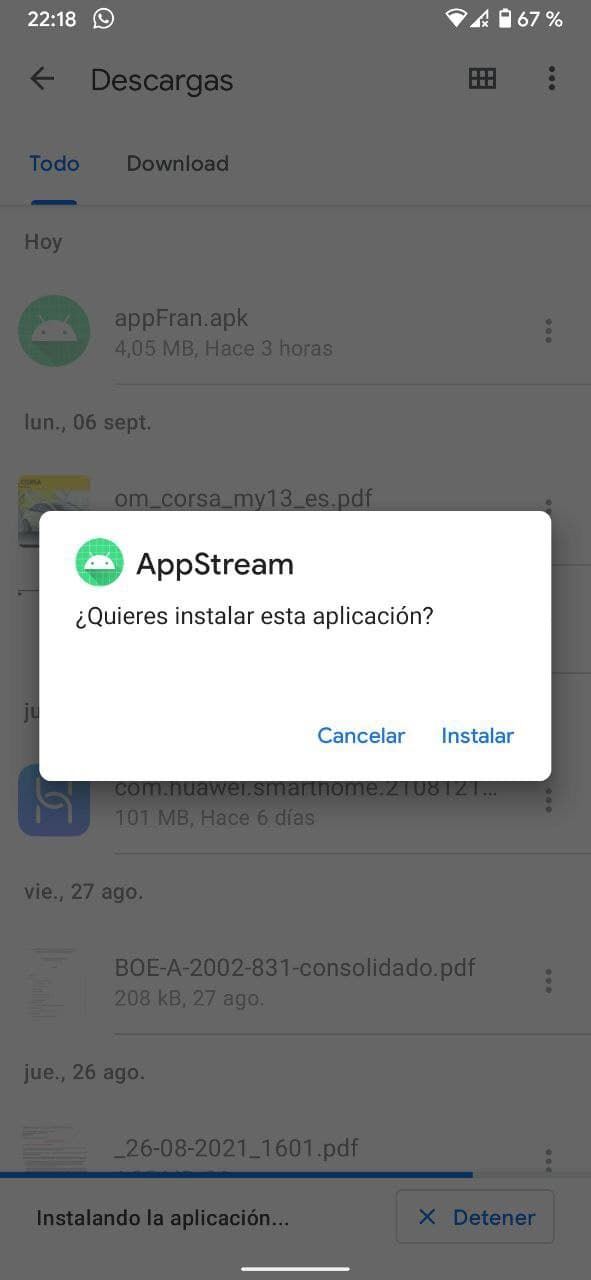
\includegraphics[width=0.35\linewidth]{img/appinstall}
	\caption{Instalación de la aplicación desde un archivo APK.}
	\label{fig:appinstall}
\end{figure}
\item
	Es posible que recibamos un aviso como el que se muestra a continuación\ref{fig:appinstall1}.\\
\begin{figure}[h!]
	\centering
	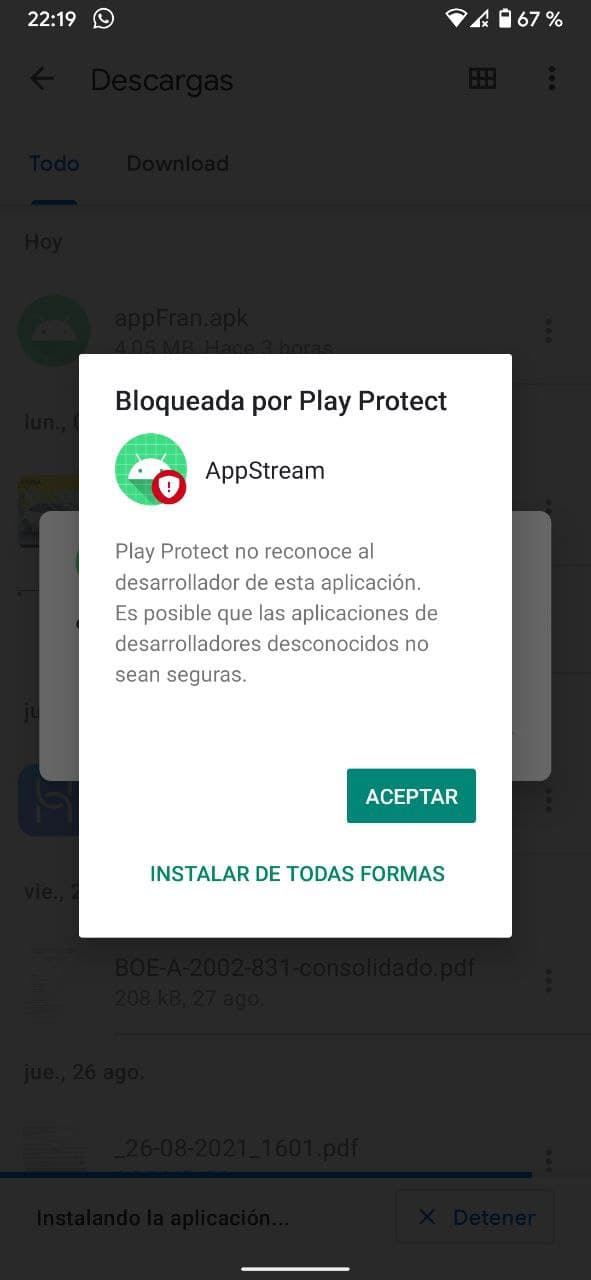
\includegraphics[width=0.35\linewidth]{img/appinstall1}
	\caption{Aviso en la instalación de la aplicación desde un archivo APK.}
	\label{fig:appinstall1}
\end{figure}
	Debemos pulsar en \textit{Instalar de todas formas}.
\end{itemize}



\section{Manual del usuario}

En este manual se va a proceder a explicar cómo hacer uso de la aplicación.

\subsubsection{Conectarse al servidor}

Para conectarnos al servidor debemos navegar hasta la pantalla \textit{Settings}.

\begin{itemize}
\item
	Desde la pantalla principal abriremos el menú de navegación en el borde superior izquierdo (\ref{fig:appmanual1}).
\begin{figure}[h!]
	\centering
	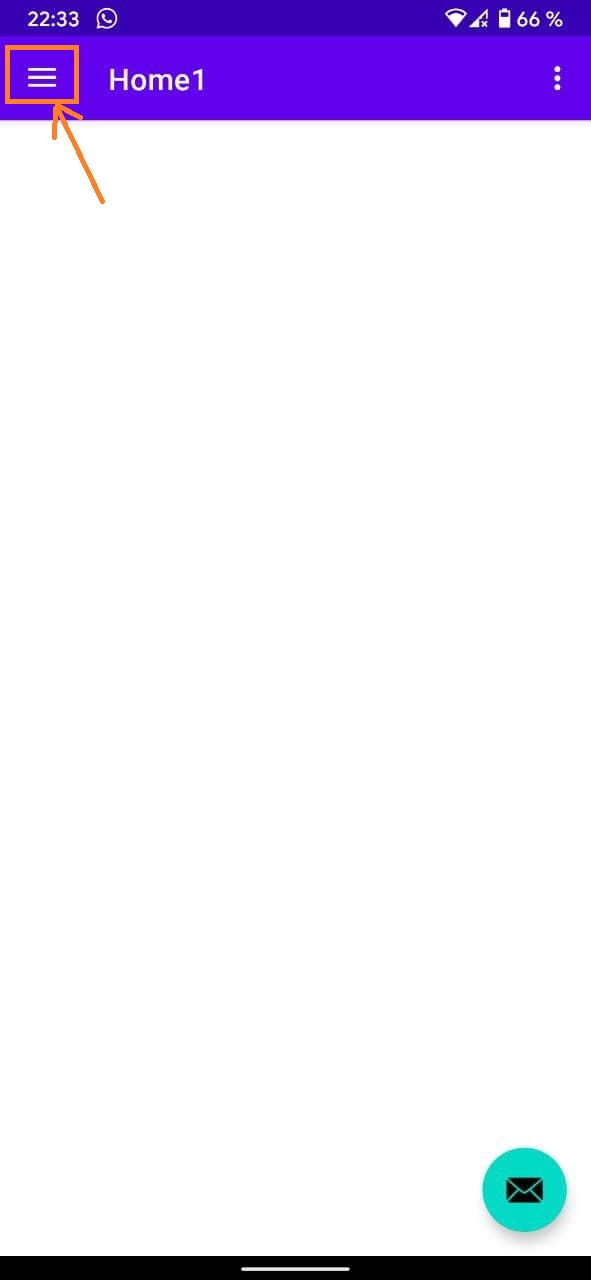
\includegraphics[width=0.35\linewidth]{img/manualuse0}
	\caption{Pantalla principal de la aplicación.}
	\label{fig:appmanual1}
\end{figure}
\item
	Desde el menú de navegación pulsaremos \textit{Settings} para ir a la pantalla de \textit{Settings} (\ref{fig:appmanual2}).
\begin{figure}[h!]
	\centering
	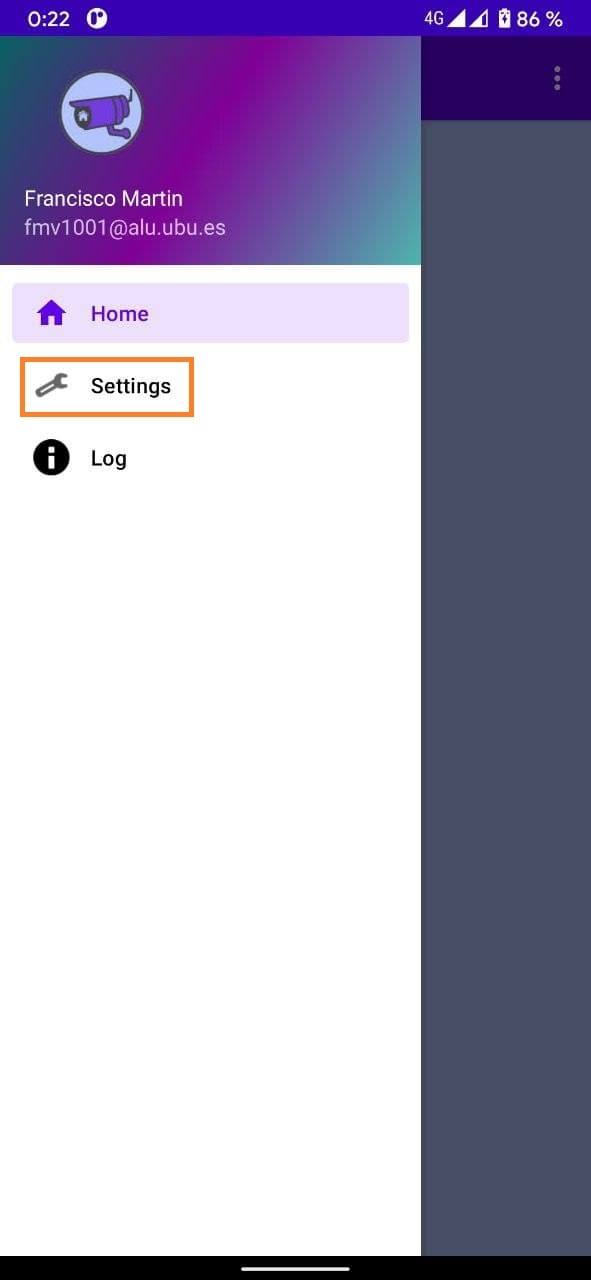
\includegraphics[width=0.35\linewidth]{img/manualuse01}
	\caption{Menú de navegación de la aplicación.}
	\label{fig:appmanual2}
\end{figure}
\item
	Una vez en la pantalla de \textit{Settings} procederemos a rellenar los campos con la Ip del servidor y el puerto de escucha (este es el 8888 por defecto) (\ref{fig:appmanual3}).
\begin{figure}[h!]
	\centering
	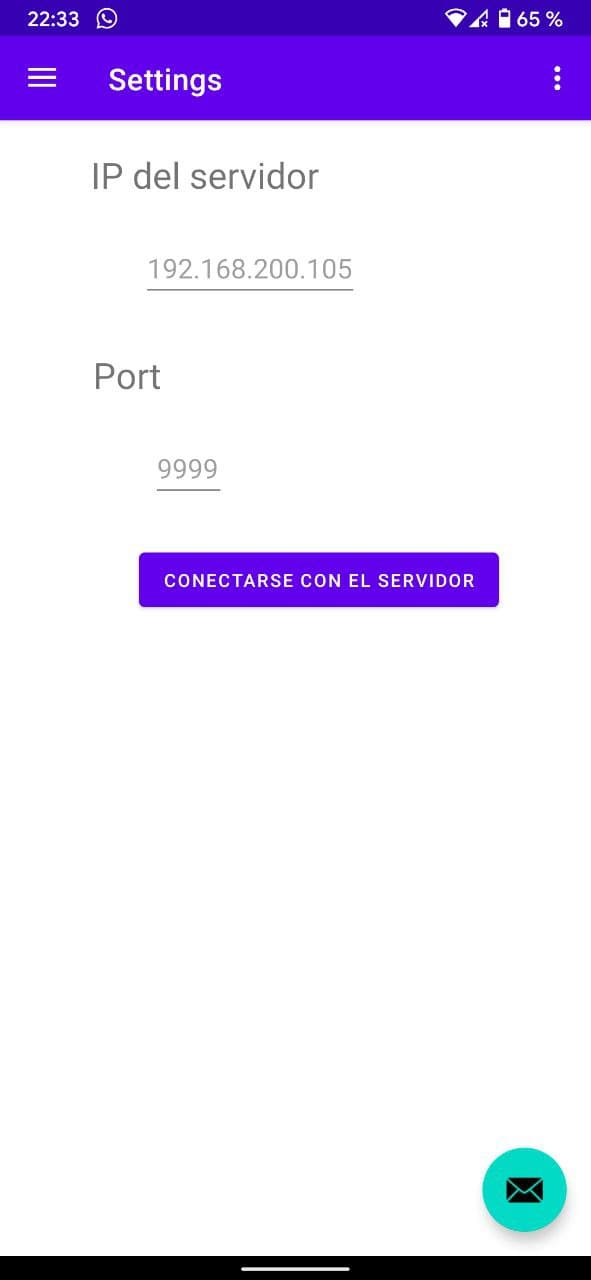
\includegraphics[width=0.35\linewidth]{img/manualuse1}
	\caption{Pantalla \textit{Settings} de la aplicación.}
	\label{fig:appmanual3}
\end{figure}
\item
	Por último pulsamos en \textit{Conectarse con el servidor}.
\end{itemize}

\subsubsection{Añadir cámara}

Para añadir una cámara debemos situarnos en la pantalla principal y abrir el menú desplegable.

\begin{itemize}
\item
	Desde la pantalla principal abriremos el menú de desplegable en el borde superior derecho (\ref{fig:appmanual4}).
\begin{figure}[h!]
	\centering
	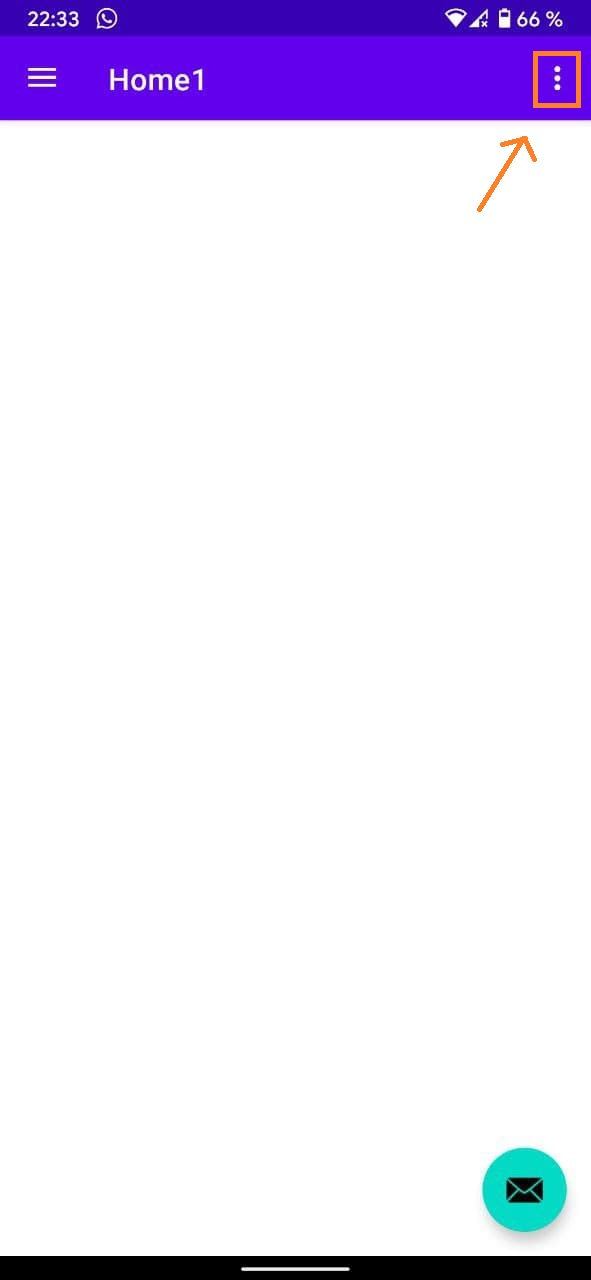
\includegraphics[width=0.35\linewidth]{img/manualuse20}
	\caption{Pantalla principal de la aplicación.}
	\label{fig:appmanual4}
\end{figure}
\item
	Desde el menú de desplegable pulsaremos \textit{Add camera} y nos saltará un cuadro de diálogo (\ref{fig:appmanual5} y \ref{fig:appmanual6}) .
\begin{figure}[h!]
	\centering
	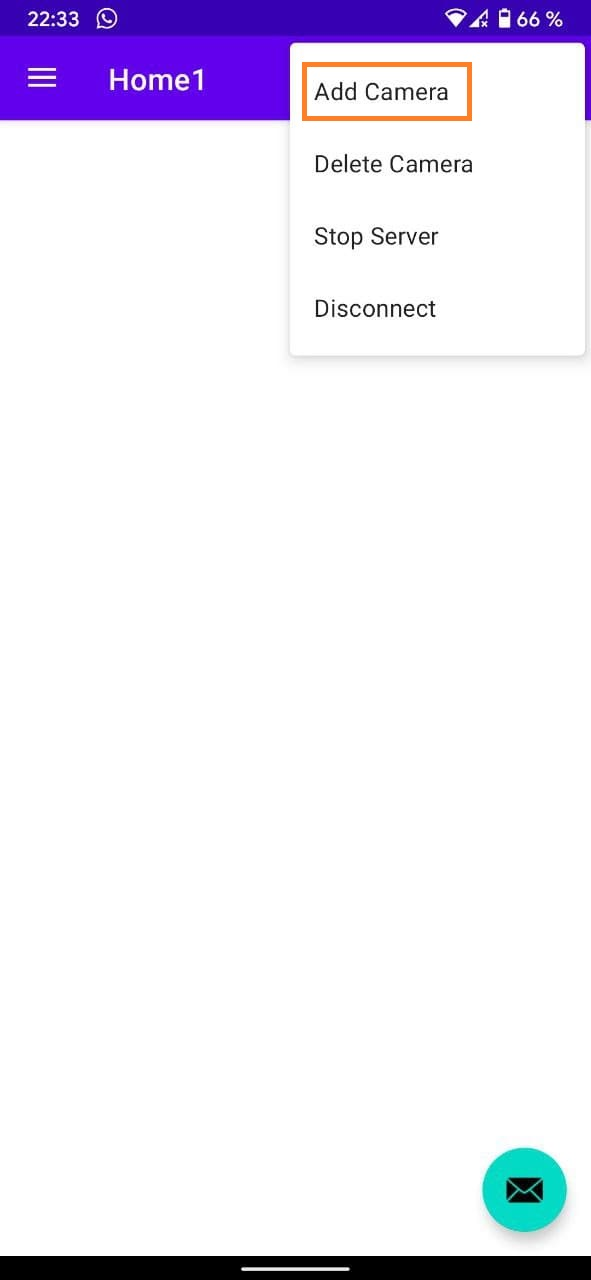
\includegraphics[width=0.35\linewidth]{img/manualuse21}
	\caption{Pantalla principal con menú desplegable abierto.}
	\label{fig:appmanual5}
\end{figure}
\begin{figure}[h!]
	\centering
	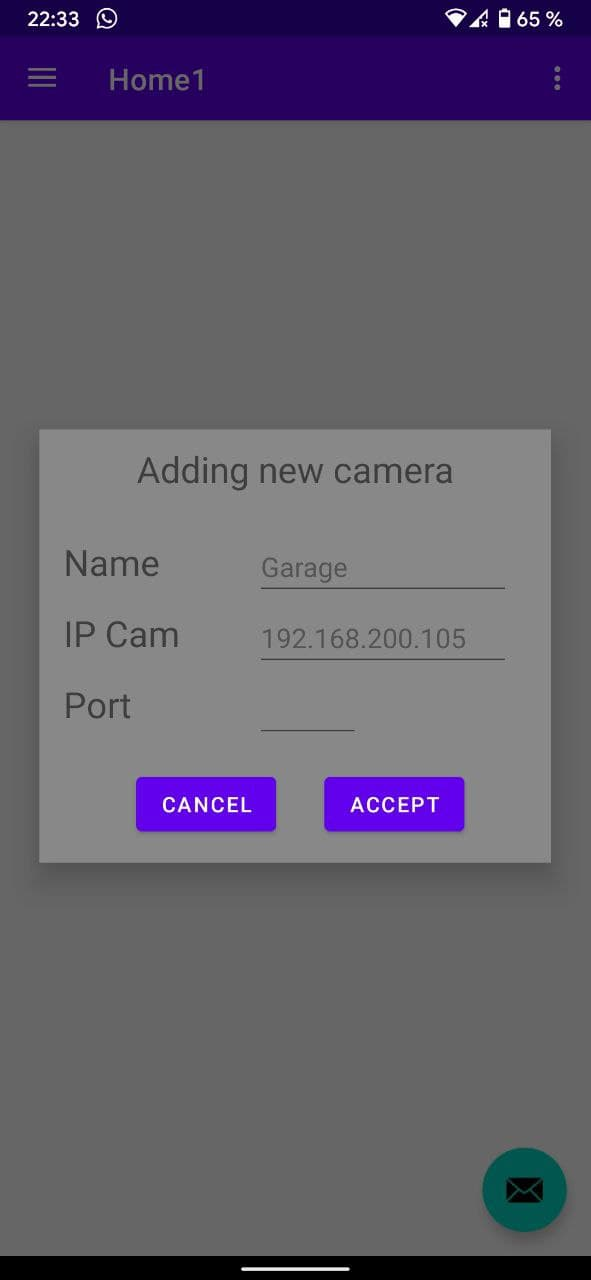
\includegraphics[width=0.35\linewidth]{img/manualuse3}
	\caption{Diálogo para añadir cámara en la aplicación.}
	\label{fig:appmanual6}
\end{figure}
\item
	Una vez en cuadro de diálogo, rellenamos los campos exigidos y hacemos clic en aceptar (\ref{fig:appmanual7}).
\begin{figure}[h!]
	\centering
	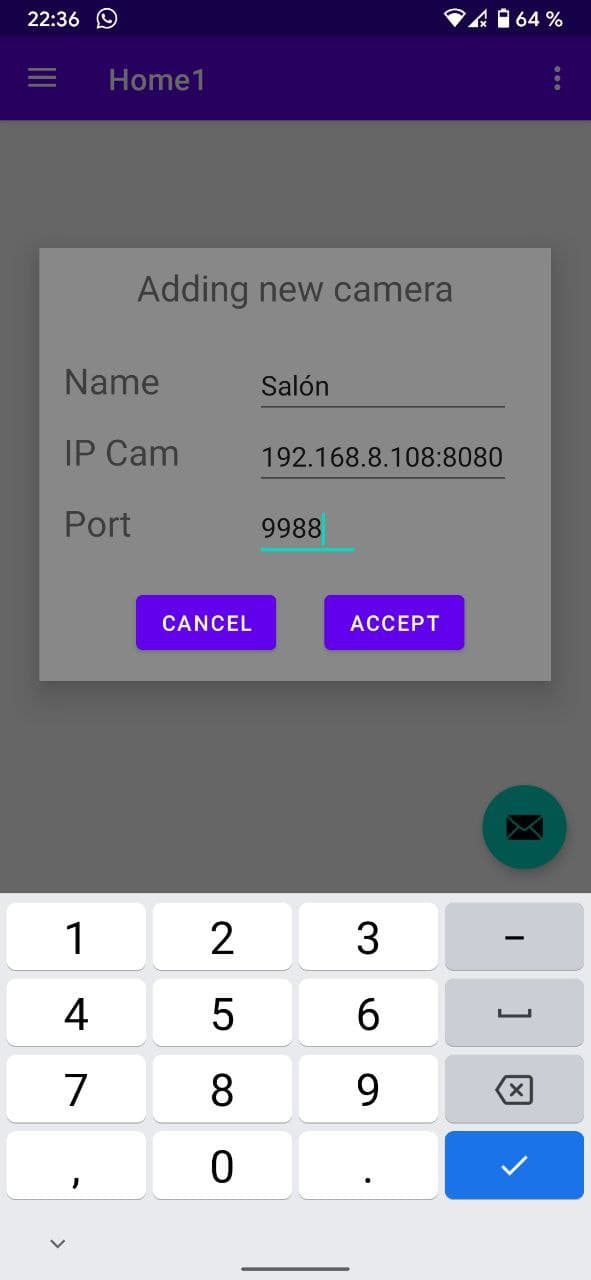
\includegraphics[width=0.35\linewidth]{img/manualuse4}
	\caption{Diálogo para añadir cámara en la aplicación.}
	\label{fig:appmanual7}
\end{figure}
\item
	Se ha mostrado en la pantalla principal el botón de la cámara introducida (\ref{fig:appmanual8}).
\begin{figure}[h!]
	\centering
	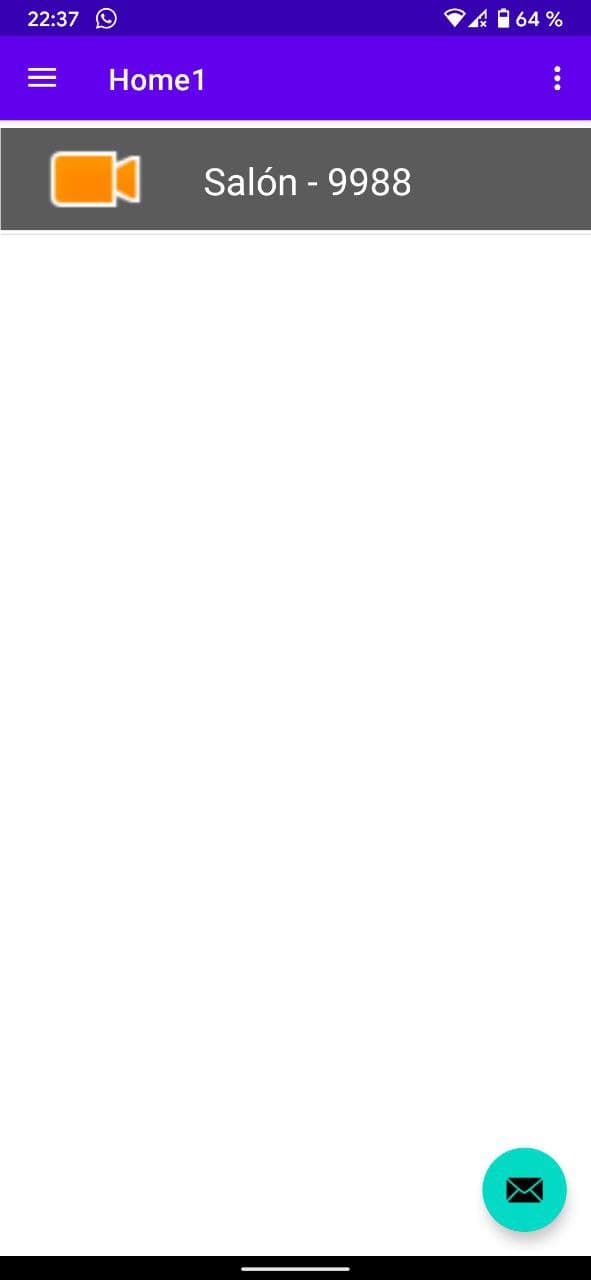
\includegraphics[width=0.35\linewidth]{img/manualuse5}
	\caption{Pantalla principal con cámara añadida en la aplicación.}
	\label{fig:appmanual8}
\end{figure}
\end{itemize}

\subsubsection{Ver cámara}

Para ver una cámara debemos situarnos en la pantalla principal y debe haber alguna ya añadida anteriormente.

\begin{itemize}
\item
	Desde la pantalla principal pulsaremos el botón de la cámara que deseemos ver, están designadas con su nombre (\ref{fig:appmanual9}).
\begin{figure}[h!]
	\centering
	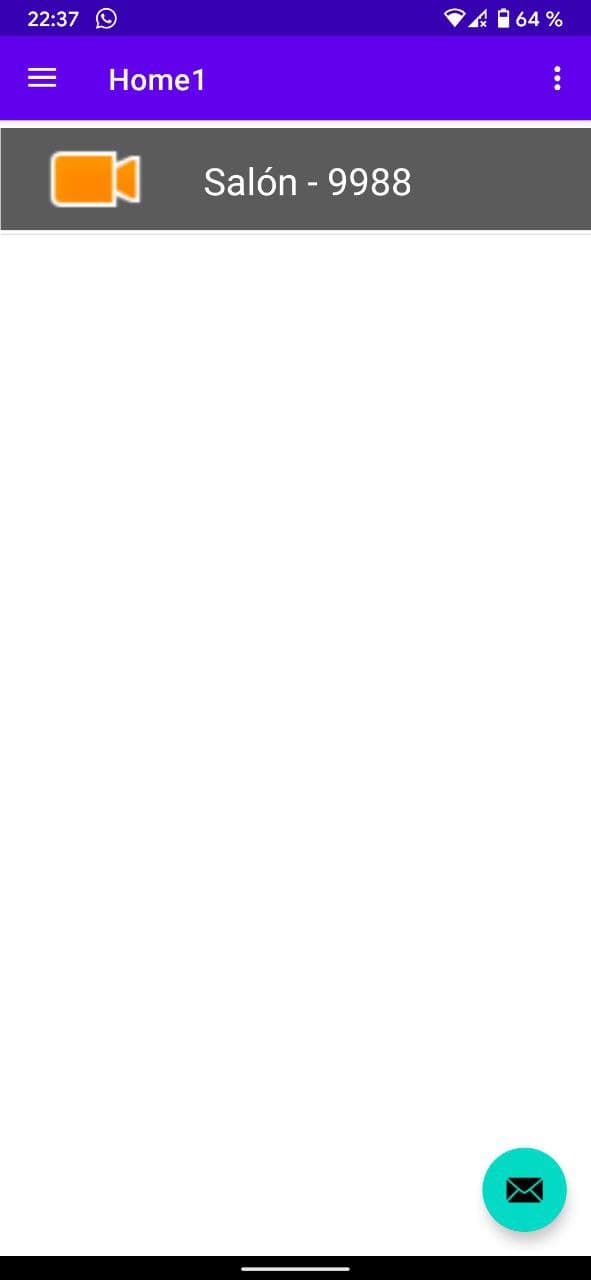
\includegraphics[width=0.35\linewidth]{img/manualuse5}
	\caption{Pantalla principal con cámara añadida en la aplicación.}
	\label{fig:appmanual9}
\end{figure}
\item
	Se nos abrirá una pantalla donde se muestra la imagen en teimpo real (\ref{fig:appmanual10}).
\begin{figure}[h!]
	\centering
	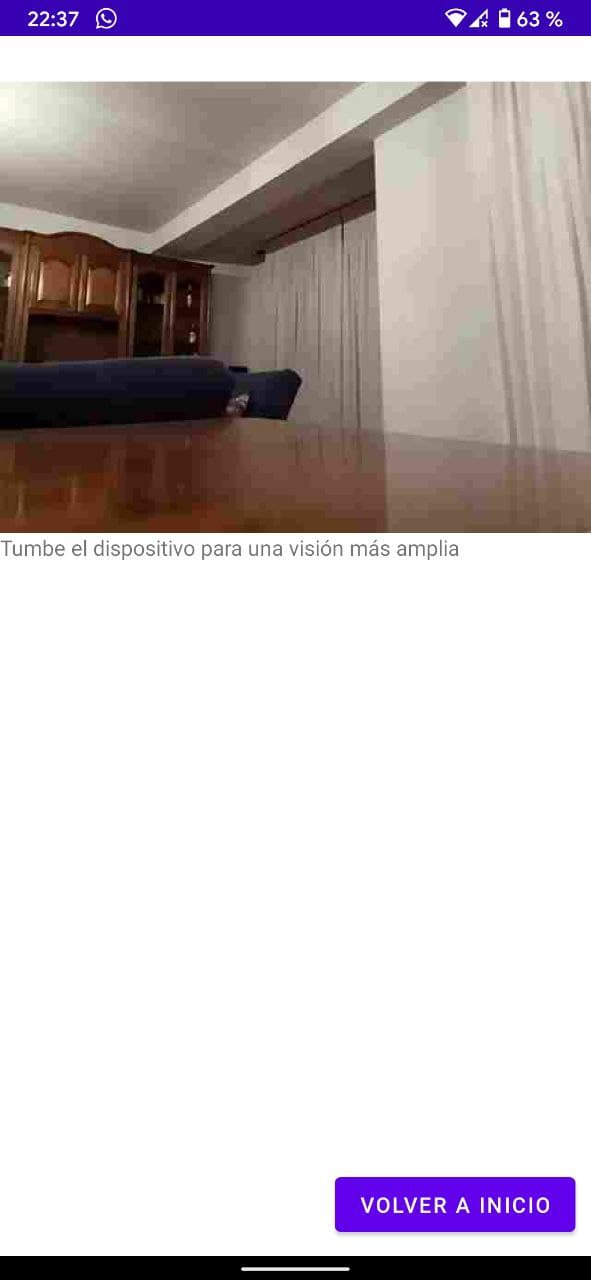
\includegraphics[width=0.35\linewidth]{img/manualuse6}
	\caption{Pantalla de visualización de cámara.}
	\label{fig:appmanual10}
\end{figure}
\item
	Si lo deseamos podemos tumbar el dispositivo para ver una imagen mas amplia (\ref{fig:appmanual11}).
\begin{figure}[h!]
	\centering
	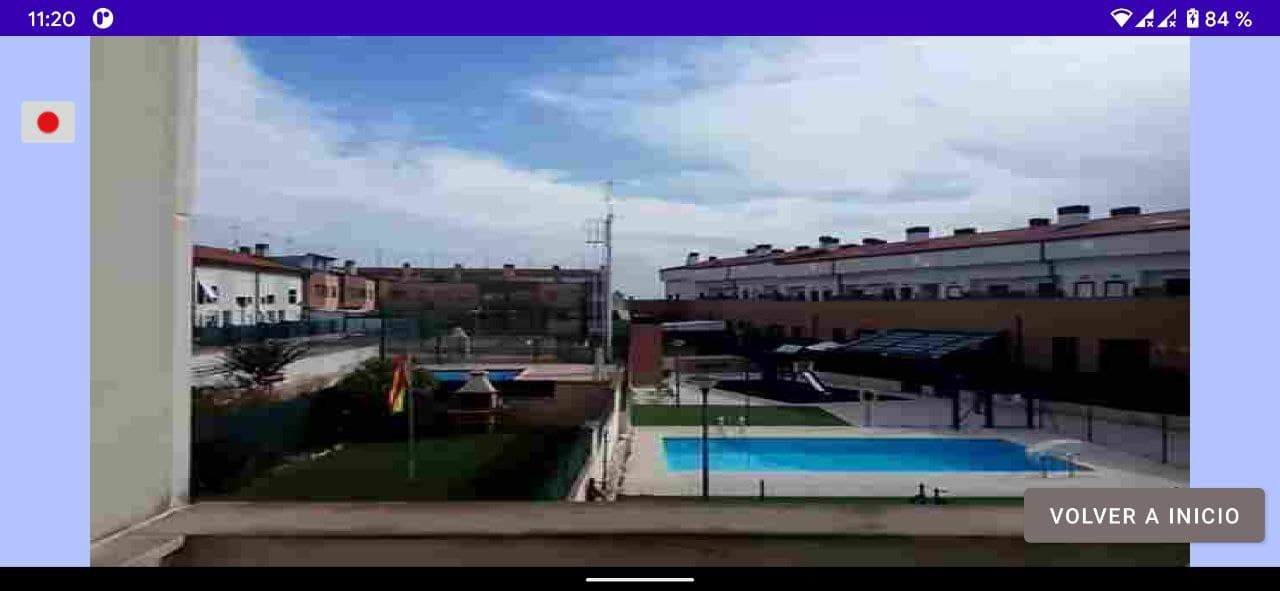
\includegraphics[width=0.9\linewidth]{img/manualuse7}
	\caption{Pantalla de visualización de cámara tumbada.}
	\label{fig:appmanual11}
\end{figure}
\end{itemize}

\subsubsection{Eliminar cámara}

Para eliminar una cámara debemos situarnos en la pantalla principal y abrir el menú desplegable.

\begin{itemize}
\item
	Desde la pantalla principal abriremos el menú de desplegable en el borde superior derecho (\ref{fig:appmanual12}).
\begin{figure}[h!]
	\centering
	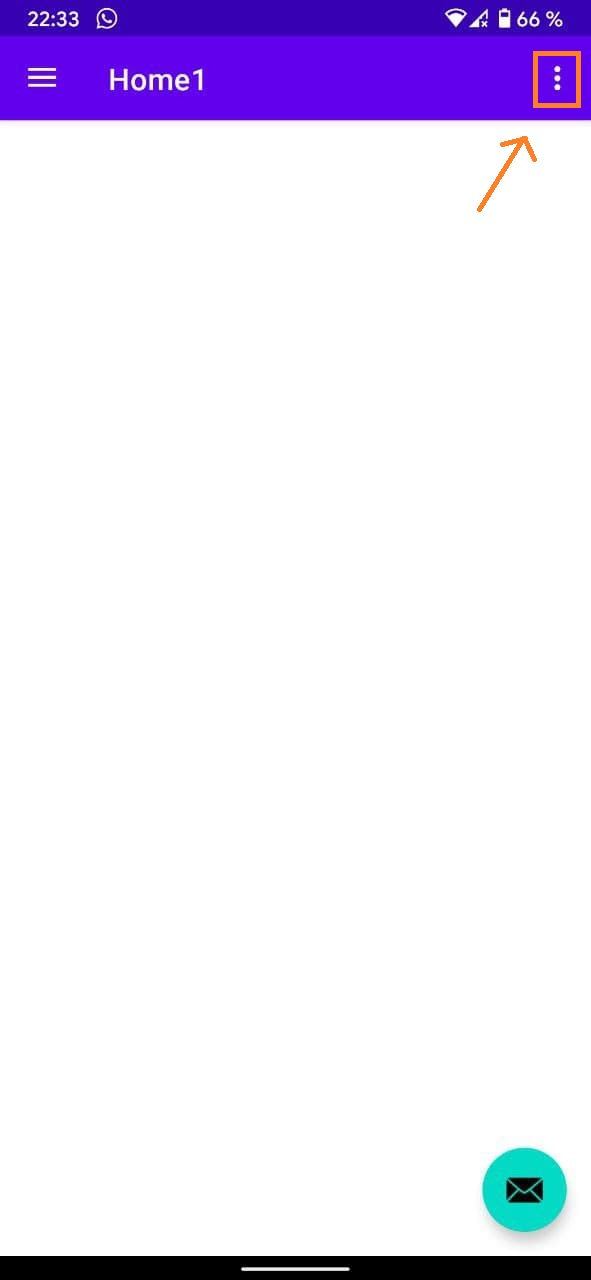
\includegraphics[width=0.35\linewidth]{img/manualuse20}
	\caption{Pantalla principal de la aplicación.}
	\label{fig:appmanual12}
\end{figure}
\item
	Desde el menú de desplegable pulsaremos \textit{Delete camera} y nos saltará un cuadro de diálogo (\ref{fig:appmanual13}).
\begin{figure}[h!]
	\centering
	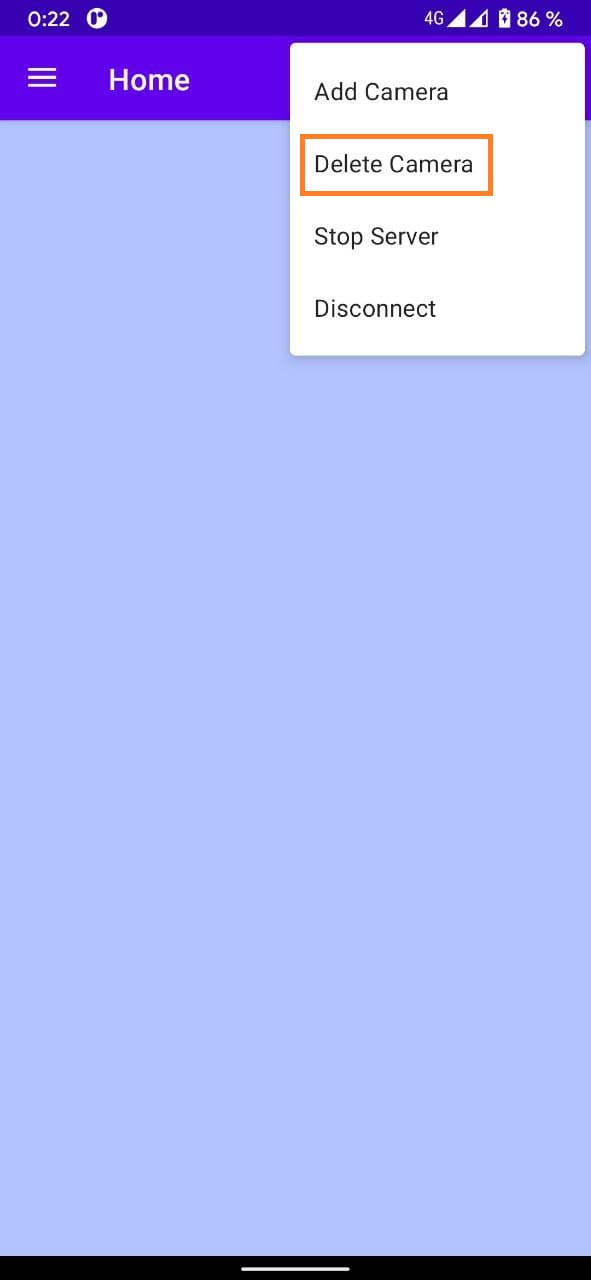
\includegraphics[width=0.35\linewidth]{img/manualuse80}
	\caption{Pantalla principal con menú desplegable abierto.}
	\label{fig:appmanual13}
\end{figure}
\item
	Una vez en cuadro de diálogo, escogemos la cámara para eliminar y hacemos clic en aceptar (\ref{fig:appmanual14}).
\begin{figure}[h!]
	\centering
	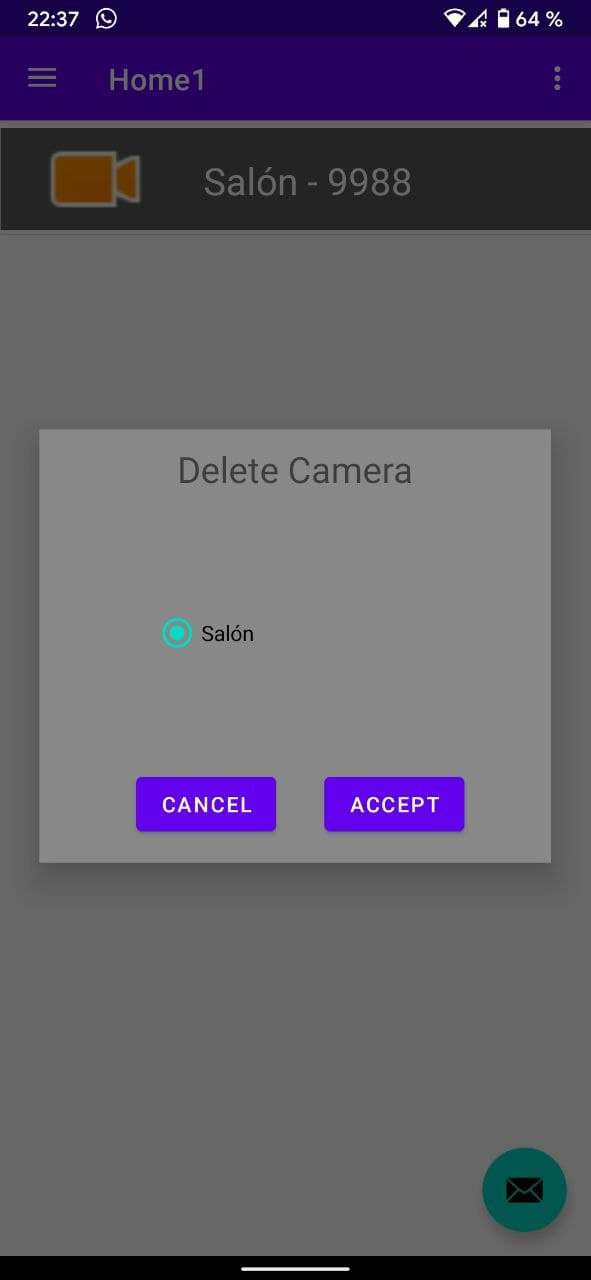
\includegraphics[width=0.35\linewidth]{img/manualuse81}
	\caption{Diálogo para eliminar cámara en la aplicación.}
	\label{fig:appmanual14}
\end{figure}
\item
	Se ha eliminado de la pantalla principal el botón de la cámara (\ref{fig:appmanual15}).
\begin{figure}[h!]
	\centering
	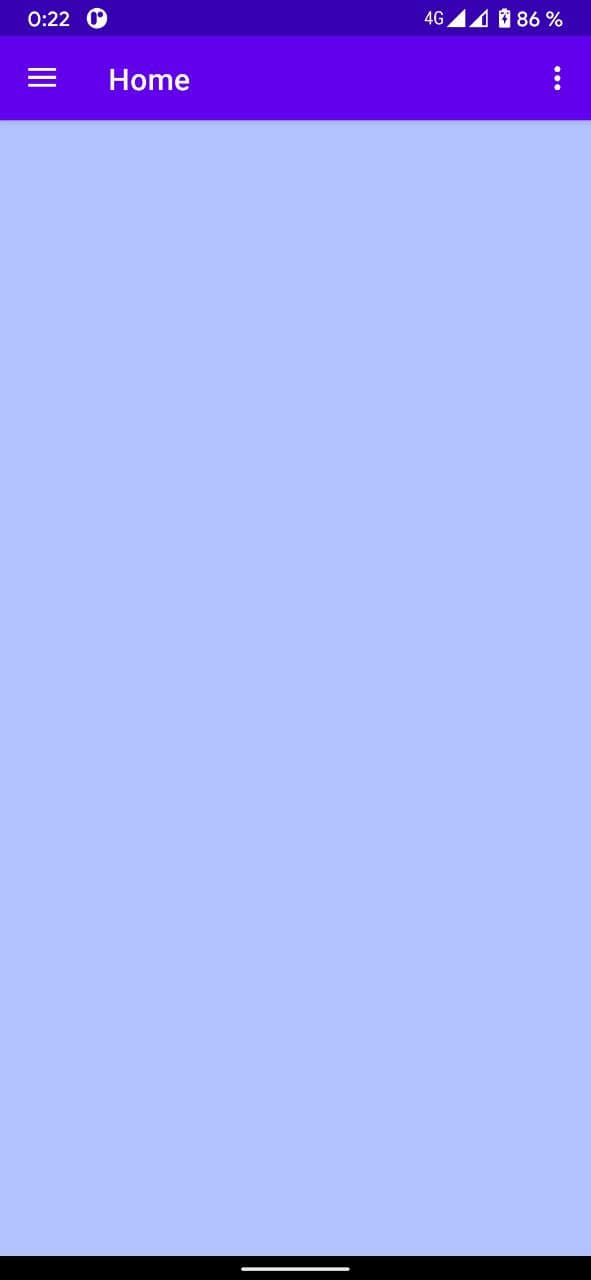
\includegraphics[width=0.35\linewidth]{img/manualuse}
	\caption{Pantalla principal con cámara eliminada en la aplicación.}
	\label{fig:appmanual15}
\end{figure}
\end{itemize}

\subsubsection{Desconectarse del servidor}

Para desconectarse del servidor debemos situarnos en la pantalla principal y abrir el menú desplegable.

\begin{itemize}
\item
	Desde la pantalla principal abriremos el menú de desplegable en el borde superior derecho (\ref{fig:appmanual16}).
\begin{figure}[h!]
	\centering
	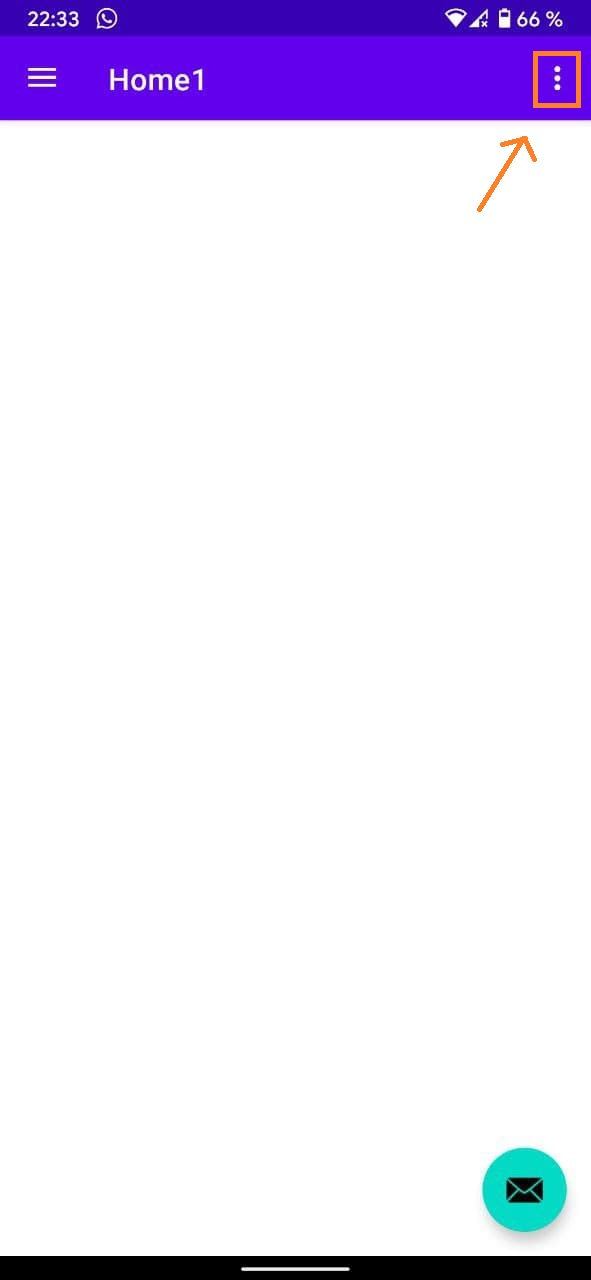
\includegraphics[width=0.35\linewidth]{img/manualuse20}
	\caption{Pantalla principal de la aplicación.}
	\label{fig:appmanual16}
\end{figure}
\item
	Desde el menú de desplegable pulsaremos \textit{Disconnect} (\ref{fig:appmanual17}).
\begin{figure}[h!]
	\centering
	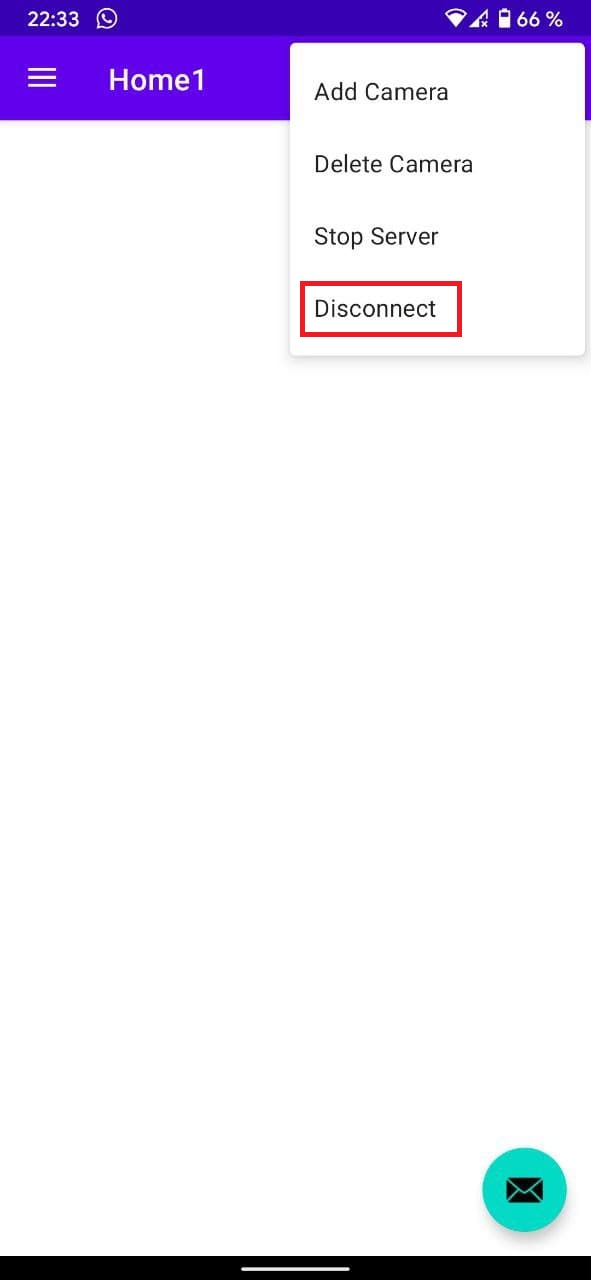
\includegraphics[width=0.35\linewidth]{img/manualuse90}
	\caption{Pantalla principal con menú desplegable abierto.}
	\label{fig:appmanual17}
\end{figure}
\end{itemize}

\subsubsection{Parar servidor}

Para parar el servidor debemos situarnos en la pantalla principal y abrir el menú desplegable.

\begin{itemize}
\item
	Desde la pantalla principal abriremos el menú de desplegable en el borde superior derecho (\ref{fig:appmanual18}).
\begin{figure}[h!]
	\centering
	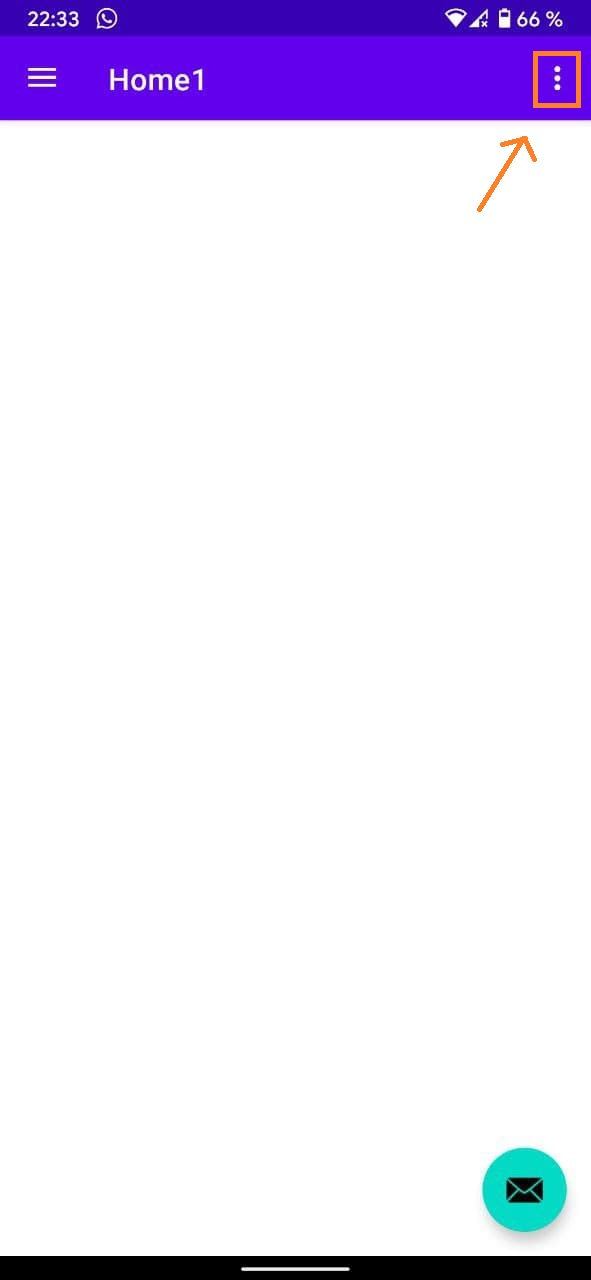
\includegraphics[width=0.35\linewidth]{img/manualuse20}
	\caption{Pantalla principal de la aplicación.}
	\label{fig:appmanual18}
\end{figure}
\item
	Desde el menú de desplegable pulsaremos \textit{Stop Server} (\ref{fig:appmanual19}).
\begin{figure}[h!]
	\centering
	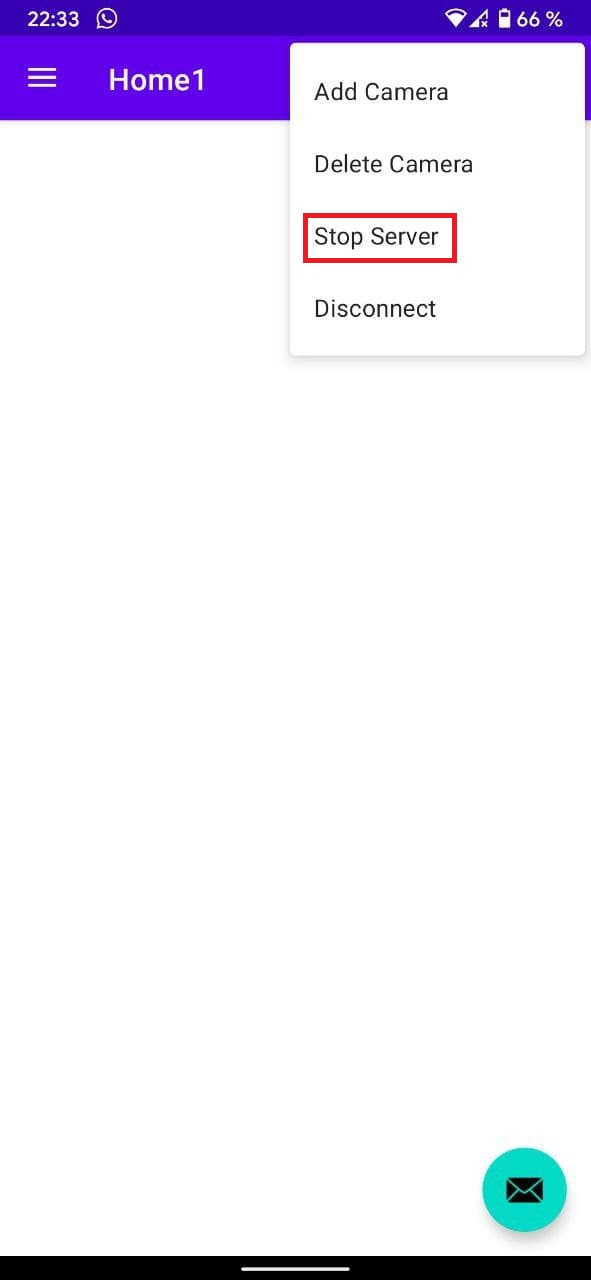
\includegraphics[width=0.35\linewidth]{img/manualuse91}
	\caption{Pantalla principal con menú desplegable abierto.}
	\label{fig:appmanual19}
\end{figure}
\end{itemize}




